%\documentclass[tikz,border=10pt]{standalone}
%\usetikzlibrary{calc,positioning}
%\usepackage{amsfonts}
%\begin{document}

\bigskip

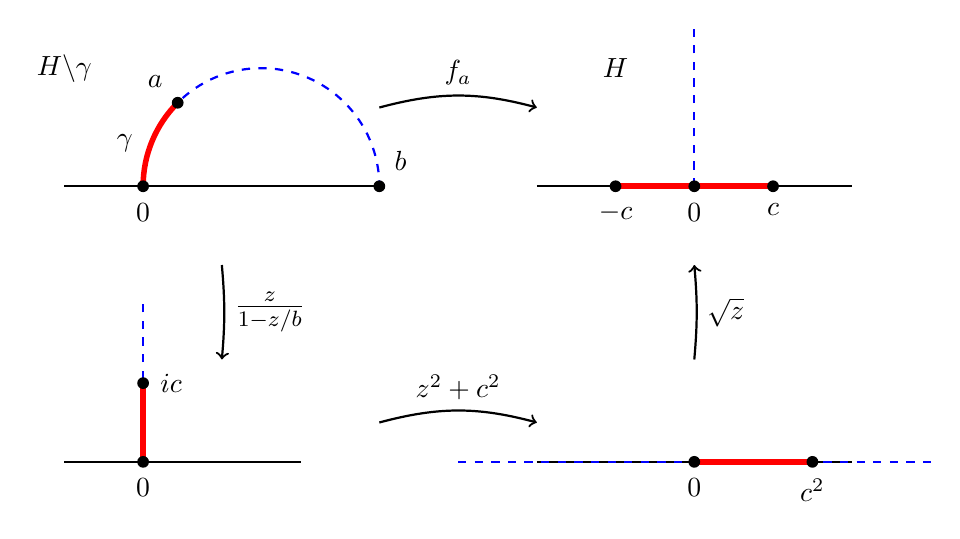
\begin{tikzpicture}[thick,
  dot/.style={fill=black,circle,inner sep=1.5pt}]

% Top left: H \ gamma
\begin{scope}[shift={(-4,2)}]
  \draw (-1,0) -- (3,0);
  \draw[dashed,blue] (0,0) arc[start angle=180,end angle=0,radius=1.5];
  \draw[red,line width=2pt] (0,0) arc[start angle=180,end angle=135,radius=1.5];
  \node[dot,label=below:$0$] at (0,0) {};
  \node[dot,label=above left:$a$] at ({-1.5*cos(45)+1.5},{1.5*sin(45)}) {};
  \node[dot,label=above right:$b$] at (3,0) {};
  \node[above left] at (0,0.3) {$\gamma$};
  \node at (-1,1.5) {$\mathbb{H}\backslash\gamma$};
\end{scope}

% Arrow from top left to top right
\draw[->] (-1,3) to[bend left=15] node[above] {$f_a$} (1,3);

% Top right: H
\begin{scope}[shift={(3,2)}]
  \draw (-2,0) -- (2,0);
  \draw[dashed,blue] (0,0) -- (0,2);
  \draw[red,line width=2pt] (-1,0) -- (1,0);
  \node[dot,label=below:$-c$] at (-1,0) {};
  \node[dot,label=below:$0$] at (0,0) {};
  \node[dot,label=below:$c$] at (1,0) {};
  \node at (-1,1.5) {$\mathbb{H}$};
\end{scope}

% Arrow from top left to bottom left
\draw[->] (-3,1) to[bend left=5] node[right, font=\large] {$\frac{z}{1-z/b}$} (-3,-0.2);

% Arrow from top right to bottom right
\draw[<-] (3,1) to[bend left=5] node[right] {$\sqrt{z}$} (3,-0.2);

% Bottom left
\begin{scope}[shift={(-4,-1.5)}]
  \draw (-1,0) -- (2,0);
  \draw[dashed,blue] (0,0) -- (0,2);
  \draw[red,line width=2pt] (0,0) -- (0,1);
  \node[dot,label=below:$0$] at (0,0) {};
  \node[dot,label=right:$ic$]at (0,1) {};
% \node[blue,right] at (0,0.5) {$ic$};
\end{scope}

% Arrow from bottom left to bottom right
\draw[->] (-1,-1) to[bend left=15] node[above] {$z^2+c^2$} (1,-1);

% Bottom right
\begin{scope}[shift={(3,-1.5)}]
  \draw (-2,0) -- (2,0);
  \draw[dashed,blue] (-3,0) -- (3,0);
  \draw[red,line width=2pt] (0,0) -- (1.5,0);
  \node[dot,label=below:$0$] at (0,0) {};
  \node[dot,label=below:$c^2$] at (1.5,0) {};
\end{scope}
\end{tikzpicture}

\bigskip

%\end{document}